% ==================================================================
% APPENDIX A1 — Hubble + r_s: extraction of ε under uniform-ε def.
%
% First per-probe methodology appendix (template for A2-A6).
% Structure: A1.1 physics / A1.2 inputs / A1.3 ECT-side model /
% A1.4 extraction procedure / A1.5 intervals / A1.6 figure /
% A1.7 limitations.
%
% Numerics source: scripts/epsilon_convergence/ch1_hubble.py,
% result_ch1.json. Figure: scripts/fig_hubble_rs_extraction.py ->
% figures/fig_hubble_rs_extraction_bw.pdf (GRAYSCALE).
%
% NO legacy "3 per cent", "ε = 0.010" narrative.
% Extraction layer only — forward machinery in app:late_cosmo_*.
% ==================================================================

\section{Extraction of the effective uniform-$\varepsilon$ interval
from the Hubble + $r_s$ channel}
\label{app:eps_extraction_hubble}

The purpose of this appendix is to set out, in one place and at the
level of detail appropriate for reproducibility, how the effective
one-dimensional $\varepsilon$-interval quoted for the Hubble + $r_s$
channel in \S\ref{subsec:eps_retained_rebuilt} is obtained. The
appendix follows the unified per-probe template also used in the
JWST, cosmic chronometer, $f\sigma_8$, and ISW extraction appendices
introduced later. The forward-modelling machinery ---
the late-time ordered-branch background, the $\varepsilon$-deformed
expansion, and the auxiliary numerical algorithms ---
is collected in Appendix~\ref{app:late_cosmo_background} and
Appendix~\ref{app:late_cosmo_algorithm}. The task of the present
appendix is the inverse step: given observational inputs and the
uniform-$\varepsilon$ ansatz, to extract the one-dimensional
$\varepsilon$-interval that this single channel admits.

\subsection*{A1.1\quad Physics of the probe}

Two independent determinations of the present-day Hubble rate are
compared. The local distance-ladder determination
$H_0^{\rm SH0ES}$ uses Cepheid-calibrated Type~Ia supernovae and is
insensitive to sound-horizon physics. The CMB-based determination
$H_0^{\rm Planck}$ is obtained from the acoustic-scale angle
$\theta_s = r_s / D_A(z_*)$, measured to high precision by the Planck
mission~\cite{Planck2018}. A shift in the inferred late-time expansion
rate can arise if the late-time gravitational response function
changes from the $\Lambda$CDM form. In the effective
uniform-$\varepsilon$ layer adopted in
\S\ref{subsec:eps_def_rebuilt}, this response is parametrised by
\begin{equation}
\frac{G_{\rm eff}(z)}{G_N} \;=\; (1+z)^{2\varepsilon}.
\label{eq:Geff_uniform_eps_A1}
\end{equation}
Under this parametrisation, both the low-redshift distance integral
(entering $H_0^{\rm Planck}$ through $D_A(z_*)$) and the high-redshift
sound-horizon integral (entering $r_s$) are modified. The channel
therefore tests $\varepsilon$ through the joint constraint imposed by
a fixed, precisely-measured $\theta_s$ and an independently determined
local $H_0$.

\subsection*{A1.2\quad Observational inputs}

The two anchoring values are
$H_0^{\rm Planck} = 67.4 \pm 0.5~\mathrm{km\,s^{-1}\,Mpc^{-1}}$
from Planck~2018 in $\Lambda$CDM and
$H_0^{\rm SH0ES} = 73.04 \pm 1.04~\mathrm{km\,s^{-1}\,Mpc^{-1}}$
from the SH0ES distance-ladder analysis~\cite{Riess2022}. The target
shift to be accommodated is therefore
\begin{equation}
\Delta H_0^{\rm obs}
\;=\; H_0^{\rm SH0ES} - H_0^{\rm Planck}
\;\approx\; 5.64~\mathrm{km\,s^{-1}\,Mpc^{-1}},
\qquad
\sigma \;=\; \sqrt{\sigma_P^2 + \sigma_{\rm SH}^2}
\;\approx\; 1.15~\mathrm{km\,s^{-1}\,Mpc^{-1}}.
\end{equation}
The acoustic-scale measurement $\theta_s = r_s / D_A(z_*)$ is taken as
fixed; the $\varepsilon$-scan is carried out at fixed $\theta_s$, such
that the $\varepsilon$-deformation modifies $r_s$ and $D_A(z_*)$ in
correlated ways.

\subsection*{A1.3\quad ECT-side model}

Under the uniform-$\varepsilon$ ansatz, the Friedmann equation is
deformed to
\begin{equation}
E_{\rm ECT}^2(z,\varepsilon)
\;=\; \Omega_r\,(1+z)^4
\;+\; \Omega_m\,(1+z)^{3+2\varepsilon}
\;+\; \Omega_\Lambda\,(1+z)^{2\varepsilon},
\label{eq:eps_friedmann_A1}
\end{equation}
with $\Lambda$CDM-best-fit values
$\Omega_m = 0.315$, $\Omega_r = 9.2\times 10^{-5}$,
$\Omega_\Lambda = 1 - \Omega_m - \Omega_r$ adopted as the background
proxy. The low-redshift distance integral is
\begin{equation}
I(\varepsilon) \;=\; \int_0^{z_*} \frac{dz}{E_{\rm ECT}(z,\varepsilon)},
\qquad z_* = 1089.80,
\end{equation}
and the sound horizon at drag epoch is
\begin{equation}
r_s(\varepsilon)
\;=\; \int_{z_{\rm drag}}^{\infty}
\frac{c_s(z)}{H_0^P\,E_{\rm ECT}(z,\varepsilon)}\,dz,
\qquad z_{\rm drag} = 1059.94,
\end{equation}
with the baryon--photon sound speed
$c_s(z) = c/\sqrt{3(1+R(z))}$, $R(z) = (3\Omega_b/4\Omega_r)(1+z)^{-1}$,
$\Omega_b = 0.0493$. At fixed $\theta_s$, the inferred $H_0$ under
$\varepsilon$-deformation becomes
\begin{equation}
H_0^{\rm inferred}(\varepsilon)
\;=\; H_0^P \cdot
\frac{I(\varepsilon)}{I(0)}
\cdot
\frac{r_s(0)}{r_s(\varepsilon)}.
\label{eq:H0_inferred_eps}
\end{equation}
For $\varepsilon > 0$, the sound-horizon integral decreases by a
larger fractional amount than the distance integral, so the ratio in
\eqref{eq:H0_inferred_eps} exceeds unity and $H_0^{\rm inferred}$ is
pushed upward --- the Hubble-tension direction.

\subsection*{A1.4\quad Extraction procedure}

The $\varepsilon$-dependent prediction for the Hubble-tension shift is
\begin{equation}
\Delta H_0^{\rm pred}(\varepsilon)
\;=\; H_0^{\rm inferred}(\varepsilon) - H_0^P.
\end{equation}
The single-parameter chi-squared for this channel is
\begin{equation}
\chi^2(\varepsilon)
\;=\;
\left[\,
\frac{\Delta H_0^{\rm pred}(\varepsilon) - \Delta H_0^{\rm obs}}
     {\sigma}
\,\right]^{\!2}.
\label{eq:chi2_hubble_eps}
\end{equation}
The best-fit value $\varepsilon_*$ is the unique root of
$\Delta H_0^{\rm pred}(\varepsilon) = \Delta H_0^{\rm obs}$ in the
physical interval $\varepsilon \geq 0$, obtained by Brent root-finding.
The $1\sigma$ and $2\sigma$ intervals are obtained from
$\Delta\chi^2 = 1$ and $\Delta\chi^2 = 4$, i.e.\ from the roots of
$\Delta H_0^{\rm pred}(\varepsilon) = \Delta H_0^{\rm obs} \pm \sigma$
and
$\Delta H_0^{\rm pred}(\varepsilon) = \Delta H_0^{\rm obs} \pm 2\sigma$
respectively.

\subsection*{A1.5\quad Derivation of $1\sigma$ and $2\sigma$ intervals}

Direct numerical evaluation of the integrals in A1.3 with the
parameters stated, using the code
\texttt{scripts/epsilon\_convergence/ch1\_hubble.py}, yields
\begin{align}
\varepsilon_*
&\;=\; 0.0323,
\label{eq:eps_hubble_central}
\\[2pt]
[\varepsilon_{\rm lo}^{1\sigma},\,\varepsilon_{\rm hi}^{1\sigma}]
&\;=\; [\,0.0267,\ 0.0376\,],
\\[2pt]
[\varepsilon_{\rm lo}^{2\sigma},\,\varepsilon_{\rm hi}^{2\sigma}]
&\;=\; [\,0.0207,\ 0.0425\,].
\end{align}
The $1\sigma$ width $\Delta\varepsilon \approx 0.0109$ inherits
approximately linearly from the combined uncertainty $\sigma$ of the
input tension. The $\varepsilon$-central value maps to a full
Hubble-tension resolution by construction, modulo the methodological
limitations of A1.7. This is the numerical content of the Hubble +
$r_s$ row of Table~\ref{tab:eps_retained_probes_rebuilt} in
\S\ref{subsec:eps_retained_rebuilt}.

\begin{figure}[H]
\centering
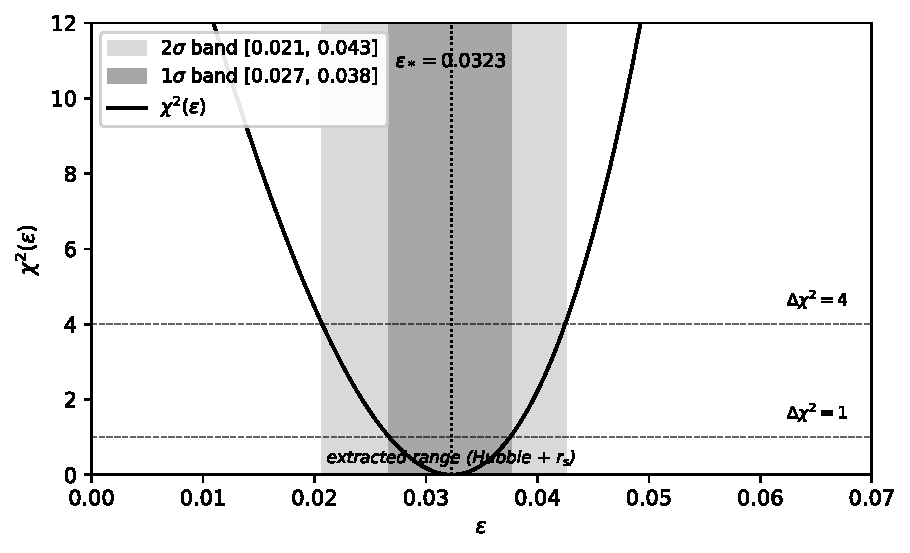
\includegraphics[width=0.78\textwidth]{figures/fig_hubble_rs_extraction_bw.pdf}
\caption{Extraction of the effective $\varepsilon$-interval for the
Hubble + $r_s$ channel. The curve shows
$\chi^2(\varepsilon)$ defined by \eqref{eq:chi2_hubble_eps}. The darker
gray band is the $1\sigma$ interval $[0.027,\,0.038]$ defined by
$\Delta\chi^2 \leq 1$; the lighter gray band is the $2\sigma$ interval
$[0.021,\,0.043]$ defined by $\Delta\chi^2 \leq 4$. The dotted vertical
line marks the best-fit $\varepsilon_* \approx 0.032$. Horizontal
dashed lines show $\Delta\chi^2 = 1$ and $\Delta\chi^2 = 4$ for
reference. All shading and line styles are grayscale per preprint
convention.}
\label{fig:hubble_rs_extraction}
\end{figure}

\subsection*{A1.6\quad Methodological limitations}

Three limitations are stated explicitly and are inherited by every
other probe of this family.

First, the background is a $\Lambda$CDM-best-fit proxy, not an
ECT-native solution; the $\varepsilon$-deformation is applied on top
of a $\Lambda$CDM parameter set taken as external input. A fully
self-consistent ECT-native extraction would use the derived
ordered-branch background of Appendix~\ref{app:late_cosmo_background}
rather than a fit obtained under a different theoretical assumption
set.

Second, the sound-horizon integral is computed with a simplified
baryon--photon sound speed $c_s(z)$, a $z_{\rm drag} = 1059.94$
anchor, and neutrino effects absorbed into $\Omega_r$. At the level
of the absolute $r_s$ this gives a few-per-cent discrepancy with the
Planck~2018 value; however, only the ratio $r_s(\varepsilon)/r_s(0)$
enters the extraction \eqref{eq:H0_inferred_eps}, and this ratio is
more robust than either absolute value.

Third, the uniform-$\varepsilon$ ansatz treats $\varepsilon$ as
epoch-independent. A first-principles $\varepsilon(z)$ from three-stage
condensate closure --- the content of OP-Hubble-derive
(\S\ref{subsec:eps_outlook_rebuilt}) --- would reshape the width of
the retained interval and in general would not map one-to-one onto a
constant $\varepsilon$. The retained interval derived here should
therefore be read as the projection of the true $\varepsilon(z)$
history onto the uniform-$\varepsilon$ diagnostic layer, not as a
measurement of a fundamental constant.

% ==================================================================
% END Appendix A1 (extraction, Hubble + r_s).
% ==================================================================
